%%===========================================================%%
%%                                                           %%
%%                       EFFICIENCIES                        %%
%%                                                           %%
%%===========================================================%%


\chapter{Efficiencies}\label{chap:efficiencies}

\section{TPC track acceptance and reconstruction efficiency}\label{sec:tpcAccAndEff}
We defined joint acceptance and efficiency of reconstruction of a track in the TPC, $\epsilon_{\textrm{\tiny TPC}}$, as the probability that particle from the primary interaction generates signal in the detector which is reconstructed as a global track that satisfies all quality criteria (cuts~\ref{sec:TpcQualityCuts}).

Thechnically this quantity was derived from single particle STARsim MC embedded into zero-bias triggers in the following procedure:
\begin{enumerate}
	\item True-level primary particles of given ID and charge were selected ($set~A$).
	\item Each particle from $set~A$ was checked if global TPC track with more than half of hit points generated by this particle was reconstructed (definition of true level particle-track matching). All global tracks which were associated with true-level primary particles and satisfied quality criteria (cut~\ref{sec:TpcQualityCuts}) formed $set~B$.
	\item The joint TPC acceptance and efficiency was calculated as the ratio of the histograms of true-level quantities (such as $p_{T}$, $\eta$, $z_{\textrm{vx}}$) for particles from $set~B$ and particles from $set~A$:
	\begin{equation}\label{eq:tpcAccAndEffDefinition}
		\epsilon_{\textrm{\tiny TPC}}\left(p_{T}, \eta, z_{vx};~\textrm{sign},\textrm{PID}\right) = \frac{(p_{T},\eta, z_{vx})~\textrm{histogram for particles of given sign and ID from}~set~B}{(p_{T},\eta, z_{vx})~\textrm{histogram for particles of given sign and ID from}~set~A}.
	\end{equation}

\end{enumerate}

The sample TPC efficiency plot is shown in Fig.~\ref{fig:tpcEff_pion_sample}. All remaining TPC efficiency plots are contained in Appendix~\ref{appendix:tpcEff}.

%---------------------------
\begin{figure}[hb]%
\centering\includegraphics[width=0.7\linewidth,page=11]{graphics/eff/Eff2D_TPC_pion_Minus.pdf}%
\caption[Sample TPC acceptance and reconstruction efficiency of $\pi^{-}$.]{Sample TPC acceptance and reconstruction efficiency of $\pi^{-}$. Plot represents the TPC efficiency $\epsilon_{\text{TPC}}$ ($z$-axis) as a function of true particle pseudorapidity $\eta$ ($x$-axis) and transverse momentum $p_{T}$ ($y$-axis) in single $z$-vertex bin whose range is given at the top. Red lines and arrows indicate region accepted in analyses.}\label{fig:tpcEff_pion_sample}
\end{figure}
%---------------------------






\section{TOF acceptance, hit reconstruction and track matching efficiency}\label{sec:tofMatchEff}

Combined TOF acceptance, hit reconstruction efficiency and matching efficiency with TPC tracks, $\epsilon_{\textrm{\tiny TOF}}$, was defined as the probability that the global TPC track that satisfy quality criteria (cuts~\ref{sec:TpcQualityCuts}) is matched with hit in TOF (matching flag of the track is different from 0). This quantity is generally referred as ``TOF efficiency''.

It was calculated in the very similiar way to TPC efficiency - single particle STARsim MC embedded into zero-bias triggers was used. Tracks belonging to $set~B$ from Sec.~\ref{sec:tpcAccAndEff} were utilized. From these tracks a sub-sample of tracks with non-zero TOF matching flag was extracted ($set~C$). The TOF efficiency was calculated as
\begin{equation}\label{eq:tofAccAndEffDefinition}
		\epsilon_{\textrm{\tiny TOF}}\left(p_{T}, \eta, z_{vx};~\textrm{sign},\textrm{PID}\right) = \frac{(p_{T},\eta, z_{vx})~\textrm{histogram for particles of given sign and ID from}~set~C}{(p_{T},\eta, z_{vx})~\textrm{histogram for particles of given sign and ID from}~set~B}.
	\end{equation}

An additional note has to be made here about the correction which is applied to TOF matching flag in MC analysis. It was found that in embedded simulation the dead TOF elements were not masked. To corect for this effect (hence obtain more reliable TOF efficiency) a data-based map of TOF modules was created, separately for each RHIC fill. Map was filled with modules which were matched with TPC tracks in the data. Each TPC track with non-zero TOF match flag in MC was then additionally checked if TOF module that it was matched with had any entries in the data-based map. If not - the TOF match flag was considered 0.

The sample TOF efficiency plot is shown in Fig.~\ref{fig:tofEff_pion_sample}. All remaining TOF efficiency plots are contained in Appendix~\ref{appendix:tofEff}.

%---------------------------
\begin{figure}[hb]%
\centering\includegraphics[width=0.7\linewidth,page=11]{graphics/eff/Eff2D_TOF_pion_Minus.pdf}%
\caption[Sample plot of TOF acceptance, reconstruction and matching efficiency of $\pi^{-}$.]{Sample plot of TOF acceptance, reconstruction and matching efficiency of $\pi^{-}$. Plot represents the TOF efficiency $\epsilon_{\text{TOF}}$ ($z$-axis) as a function of true particle pseudorapidity $\eta$ ($x$-axis) and transverse momentum $p_{T}$ ($y$-axis) in single $z$-vertex bin whose range is given at the top. Red lines and arrows indicate region accepted in analyses.}\label{fig:tofEff_pion_sample}
\end{figure}
%---------------------------

% 
% \section{TPC vertex reconstruction efficiency}\label{sec:tpcVxRecoEff}
% 
% The definition of vertex reconstruction efficiency established in this analysis is the probability that two global tracks, both associated with true-level primary particles from the kinematic region of the measurement, both satisfying kinematic and quality criteria (cuts~\ref{sec:TpcKinematicCuts} and ~\ref{sec:TpcQualityCuts}) and both matched with hits in TOF, form a vertex listed in the collection of reconstructed primary vertices and DCA(R) and DCA(z) of both global tracks calculated w.r.t. this vertex is contained within the limits of cut~\ref{sec:TpcDcaCuts}.